\documentclass[12pt]{article}
\everymath{\displaystyle}
\usepackage{unicode-math}
\usepackage{pgfplots}
\pgfplotsset{compat=1.18}
\usepackage{amsmath}



\usepackage[margin=1in]{geometry}
\usepackage{tcolorbox}
\usepackage{graphicx}
\usepackage{tikz}
\usepackage{amssymb}
\usepackage{enumitem}
\usepackage{titlesec}
\usepackage{fancyhdr}
\usepackage{pifont}
\usepackage{xcolor}
\newcounter{questionnum}
\setcounter{questionnum}{0}
\usepackage{eso-pic} % for page background

% --------- 主题颜色设置 ---------
\definecolor{novelblue}{RGB}{70,60,150}
\definecolor{headerbg}{RGB}{240,240,255}

\pagestyle{fancy}
\fancyhf{}
\renewcommand{\headrulewidth}{0.4pt}
\renewcommand{\headrule}{\hbox to\headwidth{\color{novelblue}\leaders\hrule height 0.4pt\hfill}}

% --------- 页眉背景色条 ---------
\newcommand{\headbackground}{
  \AddToShipoutPictureBG*{
    \begin{tikzpicture}[remember picture, overlay]
      \fill[blue!5!purple!10] (current page.north west) rectangle ([yshift=-60pt]current page.north east);
    \end{tikzpicture}
  }
}

% --------- 页眉设置 ---------
\pagestyle{fancy}
\fancyhf{}
\renewcommand{\headrulewidth}{0pt}
\fancyhead[L]{\color{novelblue}\textbf{\textbf{Novel Prep} }}
\fancyhead[C]{\color{novelblue}\textbf {SAT Preparation}}
\fancyhead[R]{\color{novelblue}\textbf{Jack Zeng}}


\newtcolorbox{SATCard}[1][]{%
  enhanced,
  colback=white,
  colframe=novelblue,
  coltitle=white,
  boxrule=0.6pt,
  arc=4pt,
  boxsep=5pt,
  left=8pt, right=8pt, top=10pt, bottom=10pt,
  sharp corners=south,
  drop shadow south east,
  #1
}

% --------- 顶部 Mark for Review 栏 ---------
\newcommand{\markforreview}{
  \stepcounter{questionnum} % 自动递增题号
  \begin{tikzpicture}[scale=1.1]
    % 黑色题号
    \fill[black] (0,0) rectangle (0.8,0.6);
    \node[white, font=\bfseries\large] at (0.4,0.3) {\thequestionnum};

    % 灰底主栏
    \fill[gray!10] (0.8,0) rectangle (14.5,0.6);

    % Mark for Review
    \node[anchor=west, font=\small] at (1.2,0.3) {\ding{72} \hspace{2pt}Mark for Review};

    % ABC 按钮区域
    \draw[thick, rounded corners=3pt] (13.5,0.12) rectangle (14.5,0.48);
    \node[font=\bfseries\normalsize] at (14.0,0.3) {ABC};
  \end{tikzpicture}


  \newcommand{\choiceboxcircled}[2]{%
  \begin{tcolorbox}[
    colback=white,
    colframe=black,
    boxrule=0.5pt,
    rounded corners=6pt,
    left=6pt, right=6pt, top=6pt, bottom=6pt,
    width=\linewidth
  ]
    \textbf{\large\textcircled{\textbf{#1}}} \ #2
  \end{tcolorbox}
}
}

% --------- 选项框样式 ---------
\newcommand{\choicebox}[2]{%
  \begin{tcolorbox}[
    colback=white, 
    colframe=novelblue,
    boxrule=0.5pt, 
    rounded corners=4pt, 
    left=6pt, right=6pt, top=6pt, bottom=6pt,
    width=\linewidth
  ]
  \textbf{#1.} \ #2
  \end{tcolorbox}
}


\begin{document}
\section*{Math Hard Question 7}
\noindent\markforreview
\vspace{1em}

A rectangular region of land is divided into 54 square lots of equal area \(S\) in square units. The length of the region is 1.5 times the width of the region. If the width of the region is \(a\sqrt{S}\) units, what is the value of \(a\)?

\choicebox{A}{5}  
\choicebox{B}{6}  
\choicebox{C}{7}  
\choicebox{D}{8}

\vspace{2em}

\noindent\markforreview
\vspace{1em}

In the given pair of equations, \(a\) and \(b\) are constants. The graph of this pair of equations in the \(xy\)-plane is a pair of perpendicular lines.  
Which of the following pairs of equations also represents a pair of perpendicular lines?

\[
\begin{aligned}
5x + 7y &= 1 \\
ax + by &= 1
\end{aligned}
\]

\choicebox{A}{$10x + 7y = 1$, $ax - 2by = 1$}  
\choicebox{B}{$10x + 7y = 1$, $ax + 2by = 1$}  
\choicebox{C}{$10x + 7y = 1$, $2ax + by = 1$}  
\choicebox{D}{$5x - 7y = 1$, $ax + by = 1$}

\newpage
\noindent\markforreview
\vspace{1em}

A real estate company offers a series of three webinars. 2,000 people attended the first webinar. 65\% of the people who attended the first webinar attended the second webinar, and 44\% of the people who attended both the first and second webinars attended the third webinar.

If those who attended the first but did not attend the second webinar, 31\% attended the third webinar.  
How many people attended both the first and third webinars but did not attend the second webinar?

\vspace{0.75em}

\choicebox{A}{215}  
\choicebox{B}{217}  
\choicebox{C}{219}  
\choicebox{D}{220}  

\vspace{2em}

\noindent\markforreview
\vspace{1em}

The functions \(f\) and \(g\) are defined by the given equations, where \(x \geq 0\):  
\begin{itemize}
    \item[I] \(f(x) = 19(1.27)^x + 43\)
    \item[II] \(g(x) = 8(0.77)^x\)
\end{itemize}

Which of the following equations displays, as a constant or coefficient, the maximum value of the function it defines, where \(x \geq 0\)?

\vspace{0.75em}

\choicebox{A}{I only}  
\choicebox{B}{II only}  
\choicebox{C}{I and II}  
\choicebox{D}{Neither I nor II}

\newpage
\noindent\markforreview
\vspace{1em}

Circle \(F\) in the \(xy\)-plane is represented by the equation:
\[
(x - 13)^2 + (y - 9)^2 = 196
\]
Circle \(G\) is obtained by shifting circle \(F\) 5 units to the left and 11 units up. An equation representing circle \(G\) is:
\[
(x + h)^2 + (y + k)^2 = 196
\]
where \(h\) and \(k\) are constants.  
What is the value of \(h + k\)?




\vspace{2em}

\noindent\markforreview
\vspace{1em}

The function \(q\) is defined by:
\[
q(x) = a|x - 9|^2 - 87|x - 9| + b
\]
where \(a\) and \(b\) are constants, and \(a > b > 87\).  
If \(q(639) = h\) and \(q(-621) = k\), where \(h\) and \(k\) are constants, what is the value of:
\[
9(-639)^{h-k} + 621(9)^{k-h}?
\]




\newpage
\noindent\markforreview
\vspace{1em}

In the given equation, \(a\) and \(b\) are positive constants. A solution to the equation is \(x = 42\).
\[
x(9x - 2a) + b(9x - 2a) - (x + b) = 0
\]
What is the value of \(a\)?


\vspace{2em}

\noindent\markforreview
\vspace{1em}

A right rectangular prism has a base area of \(28p\) square centimeters (\(\text{cm}^2\)). The length of the base of the rectangular prism is \(12\) cm, and the height of the rectangular prism is \(4\) cm.  
Which expression represents the surface area, in \(\text{cm}^2\), of the right rectangular prism?

\choicebox{A}{$\frac{512p}{3}$}  
\choicebox{B}{$\frac{224p}{3} + 96$}  
\choicebox{C}{$56p + 192$}  
\choicebox{D}{$560p + 96$}  

\newpage

\noindent\markforreview
\vspace{1em}

The expression
\[
\frac{x^{-2}y^{\frac{1}{2}}}{x^{\frac{1}{3}} y^{-1}}
\]
where \(x > 1\) and \(y > 1\), is equivalent to which of the following?

\choicebox{A}{$\frac{\sqrt{y}}{\sqrt[3]{x}}$}  
\choicebox{B}{$\frac{y \sqrt{y}}{\sqrt[3]{x}}$}  
\choicebox{C}{$\frac{y \sqrt{y}}{x \sqrt[3]{x}}$}  
\choicebox{D}{$\frac{y \sqrt{y}}{x^2 \sqrt[3]{x}}$}  

\vspace{2em}

\noindent\markforreview
\vspace{1em}

The function \(z\) is defined by the equation:
\[
z(w) = (0.829)^{2w}
\]
The value of \(z(w)\) decreases by \(p\%\) for each increase by 1 in the value of \(w\). Which of the following is closest to the value of \(p\)?

\choicebox{A}{0.171}  
\choicebox{B}{0.829}  
\choicebox{C}{17.1}  
\choicebox{D}{31.3}  

\vspace{2em}

\noindent\markforreview
\vspace{1em}

\[
-16(5x - 3)^2 + 4(5x - 2)^2
\]
The given expression can be rewritten as:
\[
\frac{a}{4}x^2 + \frac{b}{4}x + \frac{c}{4}
\]
where \(a, b, c\) are constants. What is the value of \(a + b + c\)?

\choicebox{A}{-112}  
\choicebox{B}{-56}  
\choicebox{C}{-28}  
\choicebox{D}{-7}  

\vspace{2em}
\newpage
\noindent\markforreview
\begin{center}
    

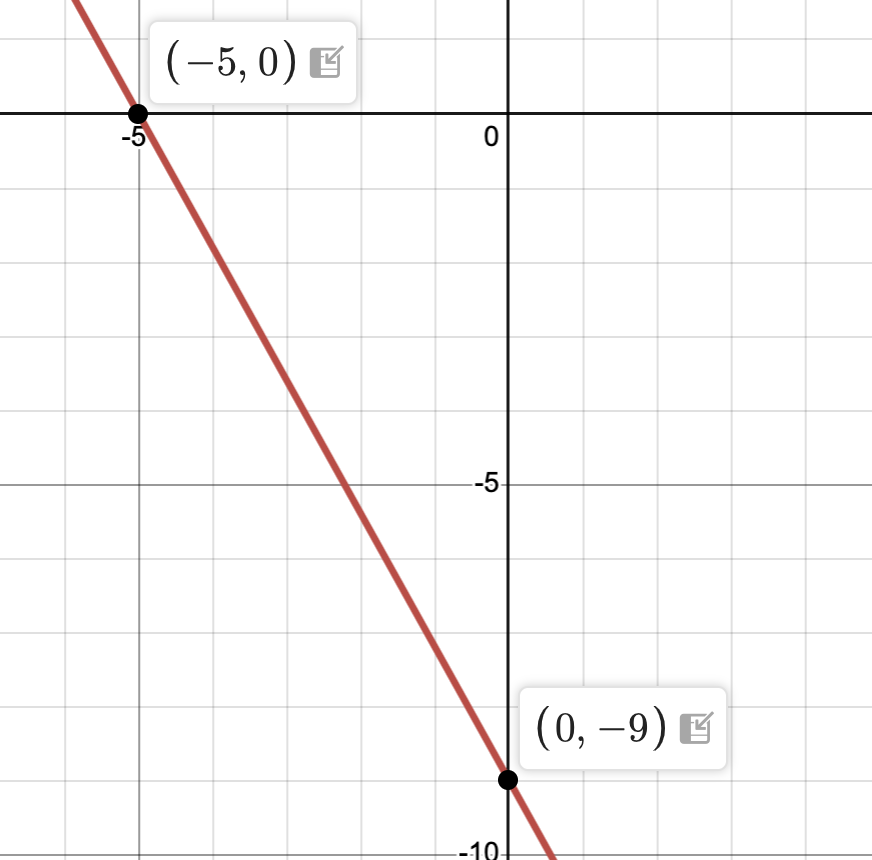
\includegraphics[width=0.4\linewidth]{f4.png}
\end{center}

The graph of line \(h\) is shown in the \(xy\)-plane. Line \(k\) (not shown) is defined by the equation:
\[
sx + 40y = t
\]
where \(s\) and \(t\) are constants. If line \(k\) is graphed in this \(xy\)-plane, the result is a graph of two linear equations. This system of two linear equations has no solution.  
Which of the following is \textbf{NOT} a possible value of \(t\)?

\choicebox{A}{-360}  
\choicebox{B}{-9}  
\choicebox{C}{72}  
\choicebox{D}{200}  






\end{document}


